% TikZ_Demo
\documentclass[dvipdfmx]{jsreport}
%\usepackage{soupreamble}
\usepackage{tikz}

\title{TikZ Demo}
%\author{M1 6012 川村聡一郎}
%\date{}


\begin{document}
\maketitle
	Notation環境


\begin{tikzpicture}[scale= 0.2]
% ページ中央
	\draw(0, 0)-- (0, 2); %
% 右ページ
	\draw(0, 0)to [out= 45, in= 135] (1.5, 0); %
	\draw(1.5, 0)-- (1.5, 2); %ページ右端
	\draw(0, 2)to [out= 45, in= 135] (1.5, 2); %
%左ページ
	\draw(-1.5, 0)to [out= 45, in= 135] (0, 0);
	\draw(-1.5, 0)-- (-1.5, 2); %ページ左端
	\draw(-1.5, 2)to [out= 45, in= 135] (0, 2);
\end{tikzpicture}

	Outline環境

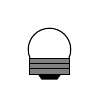
\begin{tikzpicture}[scale= 0.1]
%	scaleは0.1がちょうどいい	
	\draw(0, 0)-- (5, 0)-- (5, 2)-- (0, 2)-- cycle; %中間の相
	\fill[black](1, 0)-- (1.5, -0.7)-- (3.5, -0.7)-- (4, 0);%下のへそ
	\draw (2.5, 3.12) circle [radius= 2.7]; %上半分の半球
	\draw[fill= gray](0, 0)-- (5, 0)-- (5, 2)-- (0, 2)-- cycle; %中間層を灰色に塗りつぶした
	\draw(0, 2/3)-- (5, 2/3); %ねじ線(下)
	\draw(0, 4/3)-- (5, 4/3); %ねじ線(上)
%	\draw(1, 3)to [cute inductor] (4, 3); %フィラメント
%	\draw[line width= 1pt](1.05, 2)-- (1.05, 3); %フィラメント左足
%	\draw[line width= 1pt](3.95, 2)-- (3.95, 3); %フィラメント右足
\end{tikzpicture}

	Outline環境


\begin{tikzpicture}[scale= 0.2]
	\draw[thin](0, 0) circle [radius= 1.7];%コンパス外周
	\fill[gray](0, 0) circle [radius= 1.7];
	\draw[thin](0, 0) circle [radius= 1.5];%コンパス内周
	\fill[white](0, 0) circle [radius= 1.5];

	\fill[gray](1, 1)-- (-0.3, 0.3)-- (0.3, -0.3); %北部塗りつぶし
	\draw[thin](1, 1)-- (0.3, -0.3); %北端- 東端
	\draw[thin](1, 1)-- (-0.3, 0.3); %北端- 西端
	\draw[thin](-1, -1)-- (0.3, -0.3); %南端- 東端
	\draw[thin](-1, -1)-- (-0.3, 0.3); %南端- 西端
	\fill(0, 0) circle[radius= 0.07]; %針の中心
\end{tikzpicture}

	Remark環境

\begin{tikzpicture}
	%エクスクラメーションマーク上
	%エクスクラメーションメーク下
	%全体を囲む三角
\end{tikzpicture}

\end{document}